%!TEX root = ../documentation.tex

\chapter{Micro frontends - Fundamentals}\label{cha:Theory}

The concept behind micro frontends is similar to the widespread backend architecture microservices, but there are differences.
This is mainly because of the used environment, namely the browser, which is vastly different than clearly separated backend servers.
There are two reasons for that.
The browser \ac{API} and supported features are different between browsers.
Therefore, browser interactions are not necessarily consistent.
Secondly, while in the backend every microservice can stay separated, in the browser all applications must be composed into one application.
Depending on the composition approach, this can provide further complications.
In the browser there are four approaches to realize the micro frontend architecture.
Namely \textit{Hyperlink integration}, \textit{Build-Time integration}, \textit{Server-Side integration}, and \textit{Client-Side integration}, which are mentioned by \textcite[p.~69ff.]{Wenzel.2020} and \textcite{Leitner.2020}. %min 45:45

Before explaining the micro frontends architecture origin and its concepts, it is essential to clarify terminology synonyms first.
Depending on which literature is used, there are several terms used that mean the same thing.
Therefore, the following Table \ref{tbl:overview_synonyms} contains the terms which came up while researching micro frontend architecture.
It also outlines which terms will be used onwards in this thesis.
Also, because the term micro frontends is sometimes meant for the architecture and other times for the implementation, there is a clear separation in this thesis.
The abbreviation \ac{MF} is used for the context of an implemented frontend whereas \ac{MFA} is used for the architecture context.

The synonyms in the Table \ref{tbl:overview_synonyms} were identified based on the explanation in the references.
For example, the term \textit{shell} is mentioned by \textciteSteyer{} in the expert interview and also used in his blog post\footnotemark{}.
\footnotetext{\url{https://www.angulararchitects.io/aktuelles/micro-apps-with-web-components-using-angular-elements/} (Visited on 08/12/2020)}
In his blog he states that \enquote{[...] It contains a shell app that dynamically loads and activates micro apps. [...]}, which is the main task of a shell application.
While \citeauthorSteyer{} named it \textit{Shell}, other sources used different terms.
For example, an application named \textit{frame.js} \cite{Laug.2018} or \textit{bootstrap} \cite{Vogel.2020.Mezzalira}.
Because they all serve the same purpose, they are synonyms for the same thing.

\begin{table}[h]
    \newcolumntype{s}[1]{>{\hsize=#1\hsize}X}
    \begin{tabularx}{\linewidth}{|s{0.2}|s{0.2}|s{0.6}|}
        \hline
        \textbf{\makecell[l]{Term in \\ thesis}} &
        \textbf{Synonyms} &
        \textbf{Description}
        \\ \hline
        Shell \cite{Vogel.2020.Steyer}
                          &
        Container \cite[p.~72]{Wenzel.2020}, Frame \cite{Laug.2018} , Bootstrap \cite{Vogel.2020.Mezzalira},
        Aggregation \ac{UI} \cite{Leitner.2020}
                          &
        The application which composes the micro frontends into one application
        \\ \hline
        Hyperlink integration  \cite{Leitner.2020}
                          &
        Web approach \cite[p.~70]{Wenzel.2020}
                          &
        The integration approach where each micro frontend is one web page and they are connected via hyperlinks
        \\ \hline
        Client-Side integration \cite{Geers.2019}
                          &
        Runtime integrate \cite[p.~76]{Wenzel.2020}
                          &
        The integration approach where each micro frontend is assembled in the client browser.
        \\ \hline
        (Web) Page
                          &
        (Web) View, Screen
                          &
        One web page is related to one \ac{URL} and it can consist of one to many micro frontends
        \\ \hline
        Widget \cite{Vogel.2020.Rehm}
                          &
        Fragment \cite[p.~26]{Wenzel.2020}, Partial
                          &
        A child component of a micro frontend which can be used by other micro frontends to allow for a cross cutting page.
        \\ \hline
    \end{tabularx}
    \caption{Overview of synonyms for the \ac{MFA} and indicate which terms are used onwards in this work}
    \label{tbl:overview_synonyms}
\end{table}





\section{Evolution of web architecture}\label{cha:theory_evolution}

The origin of the \ac{MFA} is best explained by outlining the evolution of web application architecture.
Prior to \ac{MFA} there were three big iterations of architecture.
They are shown in Figure \ref{img:evolution_of_web_architecture}, which outlines the separation of responsibility between teams in regards to frontend, backend and database.
Iteration one is basically one big team which is responsible for everything and there was no code separation between frontend and backend.
The next iteration included splitting the frontend and backend code bases.
This potentially enabled providing multiple frontends for the same backend.
Over time, however, applications became even bigger, which resulted in the backend teams to grow to compensate the arising complexity \cite[p.~17f.]{Wenzel.2020}.
However, this resulted in a lower development speed, because a lot of communication is required to operate big teams.
Not only that, but also an ever growing complexity for such backends made it complex to continue working on them.
This ultimately lead to the third iteration, which is the microservice architecture.
The main intent of this architectural style is to build small autonomous services which work together \cite[p.~2]{Newman.2016}.
Also, building autonomous services provides several benefits like \cite{Leitner.2020}:
%min 4:53 

\pagebreak

\begin{enumerate}
    \item \textbf{Independent deployment}: Each microservice can be deployed without interfering other microservices
    \item \textbf{Distinct operations}: Each microservice runs, persists, and fails on its own. It should not affect other microservices
    \item \textbf{Technology agnostic}: Each microservice can use another technology if needed
    \item \textbf{Small API}: Each microservice only provides a small \ac{API} for other microservices, to keep it simple
    \item \textbf{Model around business domains}: microservices enable cutting a backend into subdomains (business needs) and each microservice is responsible for one of them. This references to the Domain Driven Design approach of software development, as a mythology of cutting domains into subdomains \cite{Evans.2004}
    \item \textbf{Parallel development}: Each microservice can be developed at the same time without interfering with others
\end{enumerate}

\begin{figure}[h]
    \centering
    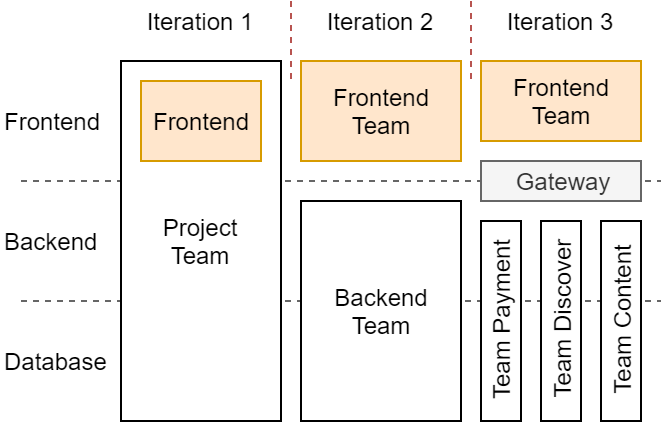
\includegraphics[scale=0.5]{evolution.png}
    \caption{Evolution of web architecture from the monolithic approach over frontend backend separation up to the microservices approach \cite[p.~17]{Wenzel.2020}}
    \label{img:evolution_of_web_architecture}
\end{figure}

These advantages resulted in a high rate of adoption of microservice architecture \cite{McCall.2019}, but it has downsides as well.
As shown in Figure \ref{img:evolution_of_web_architecture}, the server part is clearly separated into subdomains, whereas the frontend is still one big application.
The main intent of microservices is autonomy between teams, however, on the frontend side everything is  merged into one large project again, which can become a bottleneck for some projects \cite[p.~18]{Wenzel.2020}.
As a result, the mentioned benefits from the microservices architecture are lost in the frontend \cite{Leitner.2020}. %min 8:16
Consequently, the same idea of autonomy from the backend was introduced into the frontend with the \ac{MFA}, visualized in Figure \ref{img:micro_frontends_approach_detail} \cite{Geers.2019}.

Figure \ref{img:micro_frontends_approach_detail} uses the domain example shown in Figure \ref{img:evolution_of_web_architecture} and splits the frontend up.
As a result, there are independent teams which are responsible for one subdomain.
A subdomain contains all responsibilities from the frontend, over the backend and up to the database.
Consequently, it fully embraces the idea of autonomy from end to end \cite[p.18f.]{Wenzel.2020}.

\begin{figure}[h]
    \centering
    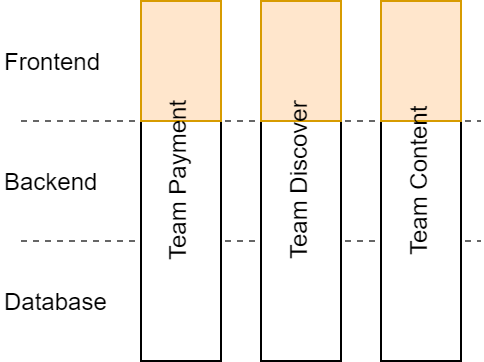
\includegraphics[scale=0.5]{mfa.png}
    \caption{Micro frontend architecture example with three teams \cite[p.~19]{Wenzel.2020}}
    \label{img:micro_frontends_approach_detail}
\end{figure}





\section{Micro frontend integration concepts}\label{cha:theory:concepts}

After explaining the origin of \acp{MF}, it is important to outline what \acp{MF} are, because there are several integration concepts.
The simplest concept is the \textit{Hyperlink integration}.
This concept utilizes hyperlinks to connect individual web pages (in this case \acp{MF}).
The advantage is that the interface surface is slim with a small complexity overhead.
However, there are disadvantages such as that only one \ac{MF} per page is allowed, transitions between \acp{MF} require roundtrips to the server and that the intercommunication between \acp{MF} is limited.
As a result, Hyperlink integration only works on a coarse grained level \cite{Leitner.2020}.
It is limited, because the only connection between the \acp{MF} is the \ac{URL}.
Hence, communication is limited to string serialized data.
Two options to transfer more complex information is via Server-Sent Events or a WebSocket connection.
Both require the backend to communicate instead \cite{Vogel.2020.Steyer}.

Concluding the \textit{Hyperlink integration}, the question remains whether the benefits mentioned beforehand in section \ref{cha:theory_evolution} are fulfilled.

\begin{itemize}
    \item Each \ac{MF} can be deployed independently from the other \acp{MF}
    \item If one \ac{MF} fails, others can continue working
    \item Each \ac{MF} can be built with a different stack
    \item Only a hyperlink connects the applications, which is the smallest interface surface possible
    \item Each \ac{MF} can be responsible for one business domain
    \item The \acp{MF} can be developed in parallel
\end{itemize}

Therefore, all benefits are met, which is also shown in the Table \ref{tbl:overview_concept_benefits} \cite{Leitner.2020}.

Besides \textit{Hyperlink integration}, there are also \textit{Build-Time integration}, \textit{Server-Side integration}, and \textit{Client-Side integration}.
These require a shell application which is responsible for integration.
Their difference lies in the time of integration \cite{Leitner.2020}.
In Figure \ref{img:container_application_concepts} the time differences are visualized.

\begin{figure}[h]
    \centering
    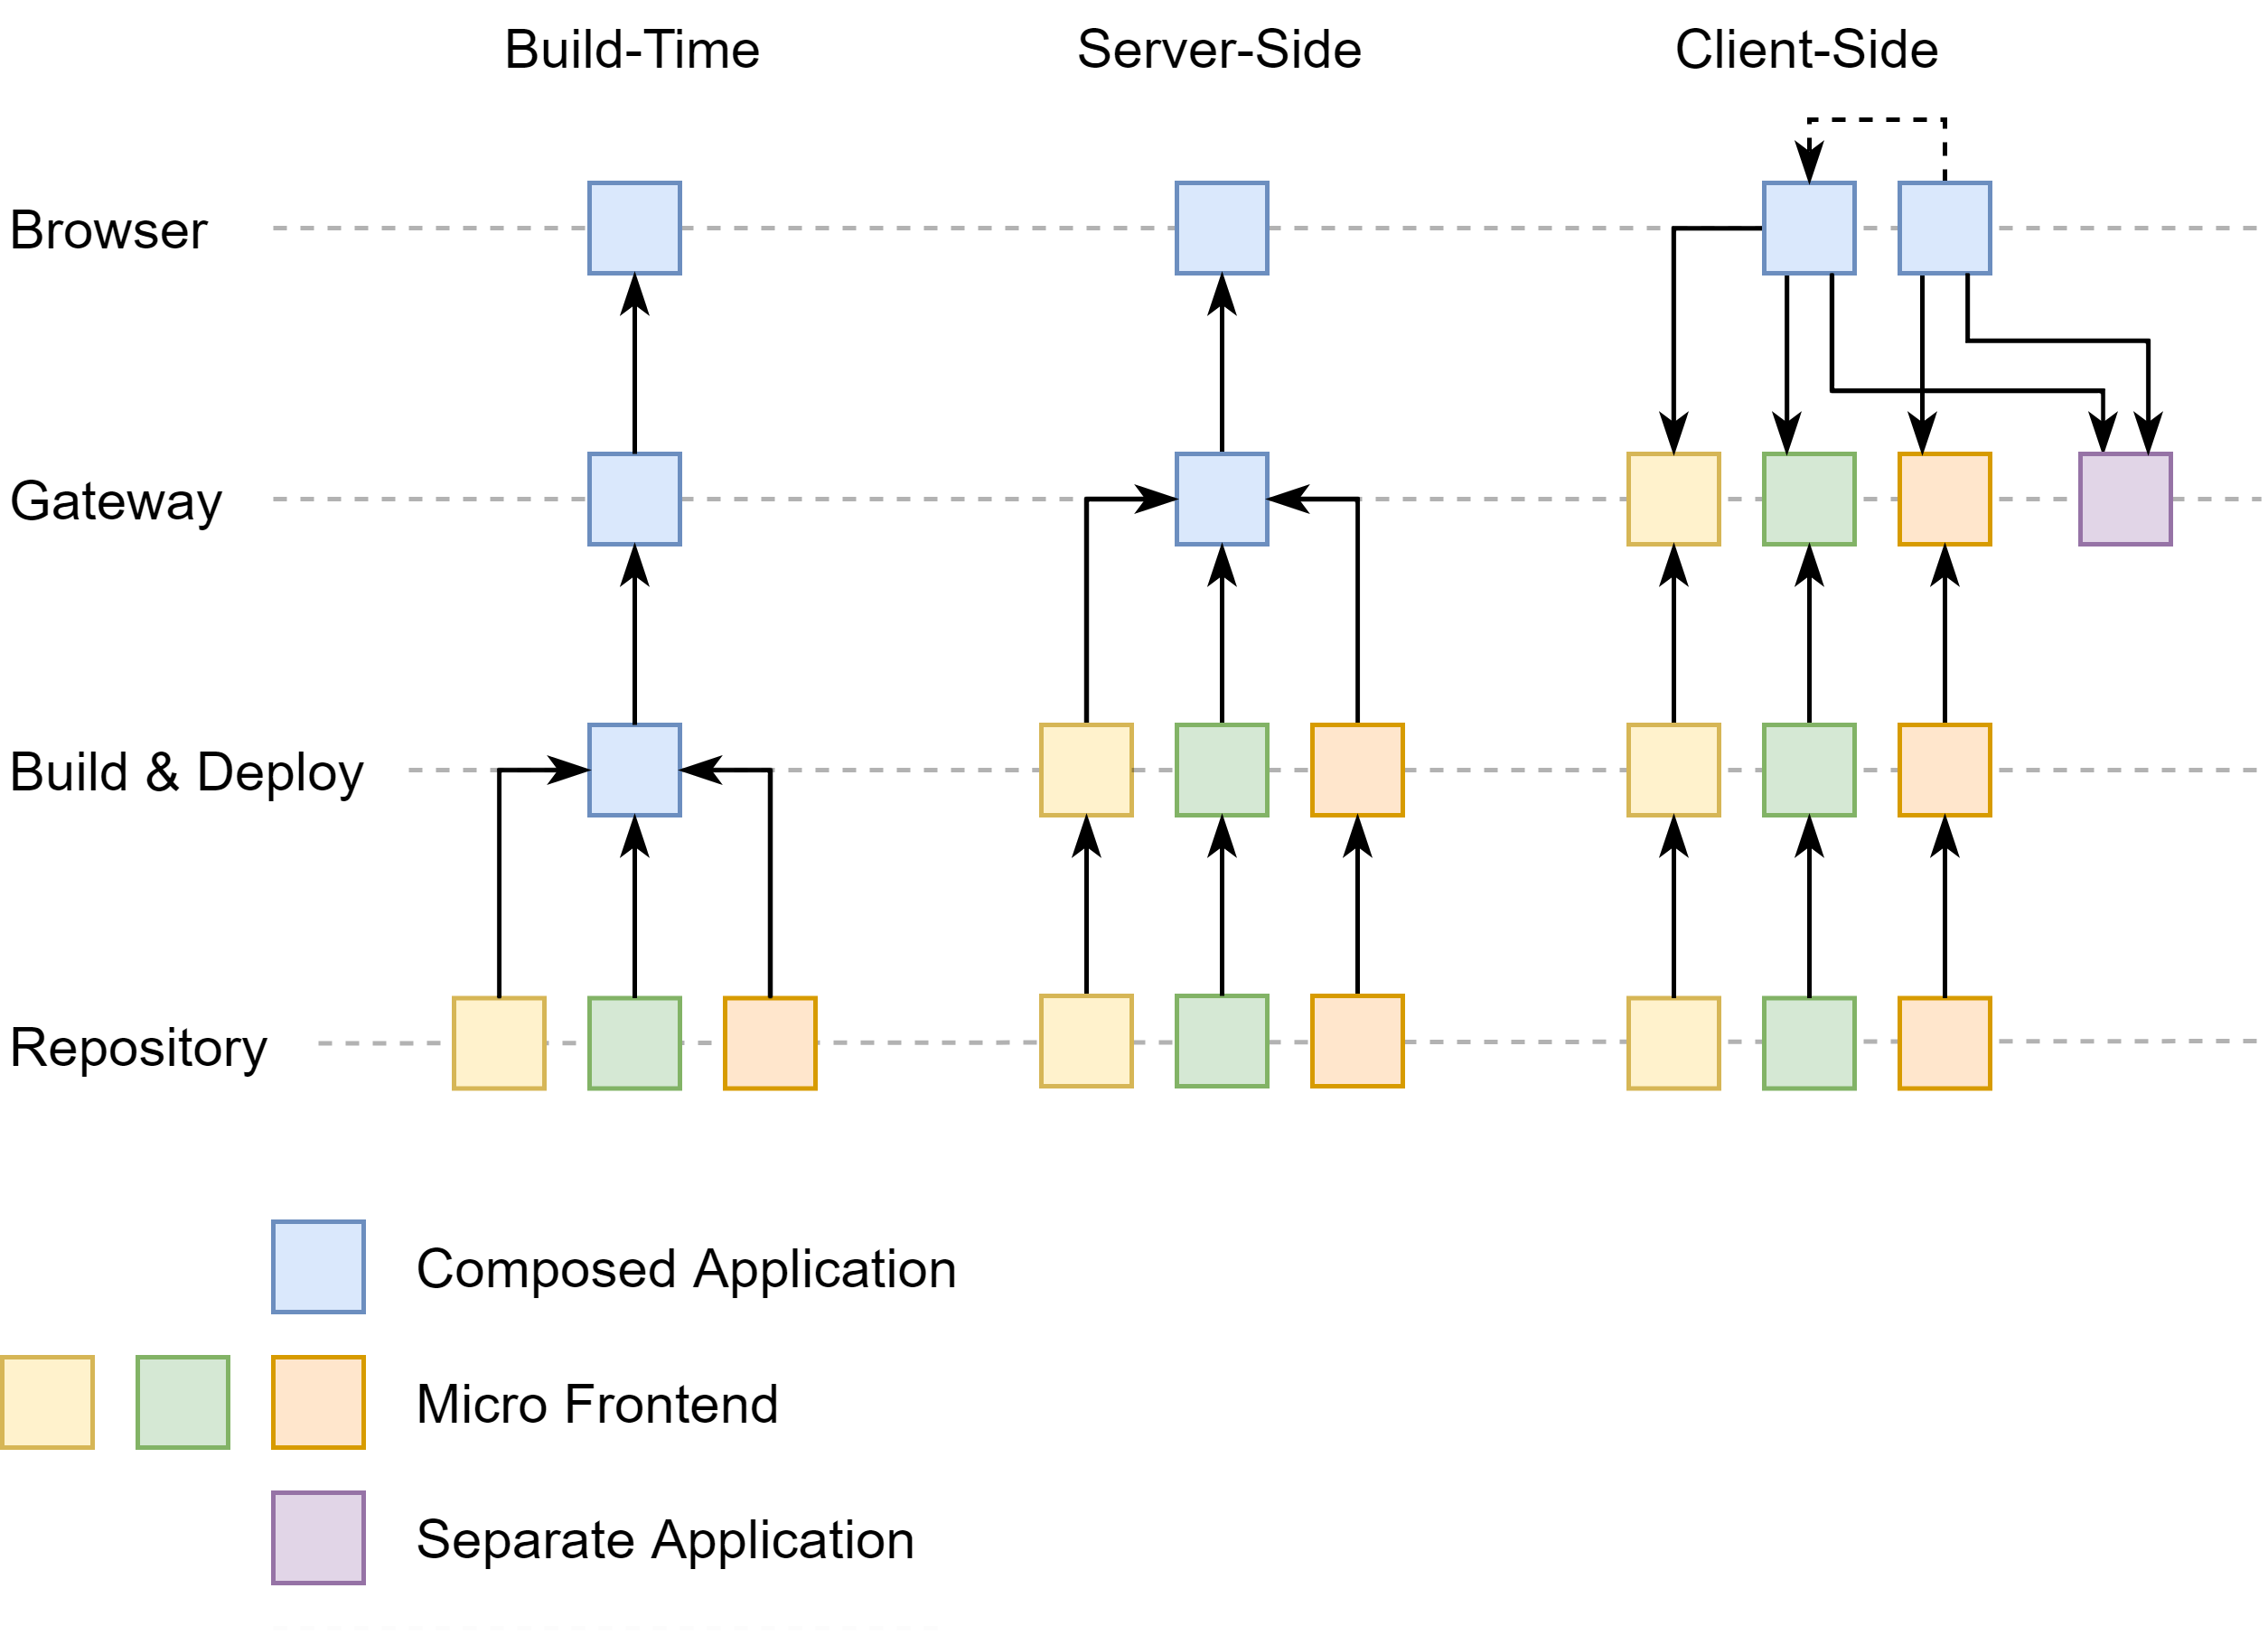
\includegraphics[width=\textwidth, keepaspectratio]{integration.png}
    \caption{Different shell application integration concepts in comparison to each other \cite{Leitner.2020}}
    \label{img:container_application_concepts}
    %min 22:50
\end{figure}

The first concept is \textit{Build-Time integration} and it is the earliest integration.
Each \ac{MF} is developed on their own, but they are combined to one application while building the application.
As a result, if any \ac{MF} is changed, then the entire application needs to be redeployed.
Hence, there is no independent deployment.
Another benefit which is missing is distinct operations.
It is very likely, that the entire application breaks if one \ac{MF} breaks.
Finally, the \acp{MF} needs to use the same technology stack in order to be built together into one application.

On the other hand, the \textit{Build-Time integration} concept allows for a small interface surface by dividing the application into separate components and \acp{MF}.
This concept also includes modeling around business domains and parallel development.
A comparison of the benefits to other concepts is shown in Table \ref{tbl:overview_concept_benefits} \cite{Leitner.2020}.

The next concept is \textit{Server-Side integration}.
Its main difference is, that each \ac{MF} is developed, built and deployed on their own and then connected before it leaves the server.
A typical approach is to use Edge-Side Includes to compose the final web page together in the gateway (i.e. the \enquote{edge}).
Contrary to the \textit{Build-Time integration}, each \ac{MF} is independent deployable.
Similarly are the distinct operations, because there are fallback solutions, if a Edge-Side Include is not available.
Also, because the composition part is about stitching together \ac{HTML} pieces, the \acp{MF} are technology agnostic.
Apart from these benefits, the other benefits apply as well, which are a small interface surface, being able to model around business domains and parallel development.
This is also shown in the Table \ref{tbl:overview_concept_benefits}.
The only disadvantage is, that it requires a lot of roundtrips to the server.
This also breaks an Single-Page Application concept.
Depending on the project this aspect can be a disadvantage or not.
It has the benefit of slim client-side applications, because less \ac{JS} is needed to compose the application client-side \cite{Leitner.2020}.

Finally, there is the \textit{Client-Side integration} concept, which is the relevant concept for this thesis.
It follows the same principles of the \textit{Server-Side integration}, but moves the integration into the client-side.
This results in also providing all benefits, which is shown in Table \ref{tbl:overview_concept_benefits}.
For this concept, a shell application is firstly loaded into the browser.
The shell is then responsible to load the needed \acp{MF} per page and integrate them.
Because the shell loads what it needs, the arrows are inverted in the Figure \ref{img:container_application_concepts} for the last step between the browser and gateway.
Also, each \ac{URL} is composed of different \acp{MF}, which results in multiple potential combinations.
This is outlined in the Figure by showing multiple \textit{Composed Applications} in the browser, which are connected via an arrow, representing the routing between them.
The final difference is, that this concept allows to integrate third-party applications.
This is hinted in the Figure by the \textit{Separate Application} which is integrated in the composed application.

\begin{table}[h]
    \begin{tabular}{|l|l|l|l|l|}
        \hline
                             &
        \textbf{Hyperlink}   &
        \textbf{Build-time}  &
        \textbf{Server-side} &
        \textbf{Client-side}
        \\ \hline
        \makecell[l]{Independent                                         \\ deployment}   & \cmark{} & \xmark{} & \cmark{} & \cmark{} \\ \hline
        Distinct operations  & \cmark{} & \xmark{} & \cmark{} & \cmark{} \\ \hline
        Technology agnostic  & \cmark{} & \xmark{} & \cmark{} & \cmark{} \\ \hline
        \makecell[l]{Small interface                                     \\ surface}& \cmark{} & \cmark{} & \cmark{} & \cmark{} \\ \hline
        \makecell[l]{Model around                                        \\ business domains} & \cmark{} & \cmark{} & \cmark{} & \cmark{} \\ \hline
        Parallel development & \cmark{} & \cmark{} & \cmark{} & \cmark{} \\ \hline
    \end{tabular}
    \caption{Overview of benefits per integration concept \cite{Leitner.2020}}
    \label{tbl:overview_concept_benefits}
\end{table}

To sum up this section, there are several approaches available to realize \ac{MFA}.
\textit{Hyperlink integration} is the simplest approach, but it is only suited for applications with fully verticalized systems.
Next up is \textit{Build-Time integration}.
Even though it does not provide all benefits, it can be a pre \ac{MFA} step in development \cite{Vogel.2020.Olleck}.
Finally, there are \textit{Server-Side integration} and \textit{Client-Side integration}.
Both provide all benefits and it comes down to the project needs, which concept is used in the end.
A final thought is not about the \ac{MFA}, but rather the fact that all these benefits come at the cost of complexity.
Each benefit mentioned comes with a complexity cost and it depends on a project which benefits are actually worth the cost.
This was mentioned by \textcite{Leitner.2020} and \textcite{Jackson.2019}.





\section{Micro frontend conceptual extensions}

After explaining the general integration concepts, there are also extensions to them which can be used if needed.
It is important to note, that from here on the practices are explained in context of \textit{Client-Side integration}.



\paragraph{\acl{BFF}}\label{cha:theory_extensions_bff}

The first conceptual extension is the architecture \acf{BFF} from the microservices architecture pool.
Normally this is used to reduce the responsibility of the \textit{\ac{API} gateway} in case that there are multiple client applications using the same backend.
To achieve the responsibility reduction, instead of using one \ac{API} gateway for all applications, it is split so that each client application uses a different \ac{API} gateway \cite[p.~69f.]{Bruce.2019}.
But before applying the \ac{BFF} to the \ac{MFA}, it is essential to outline the scenario without it.

\begin{figure}[h]
    \centering
    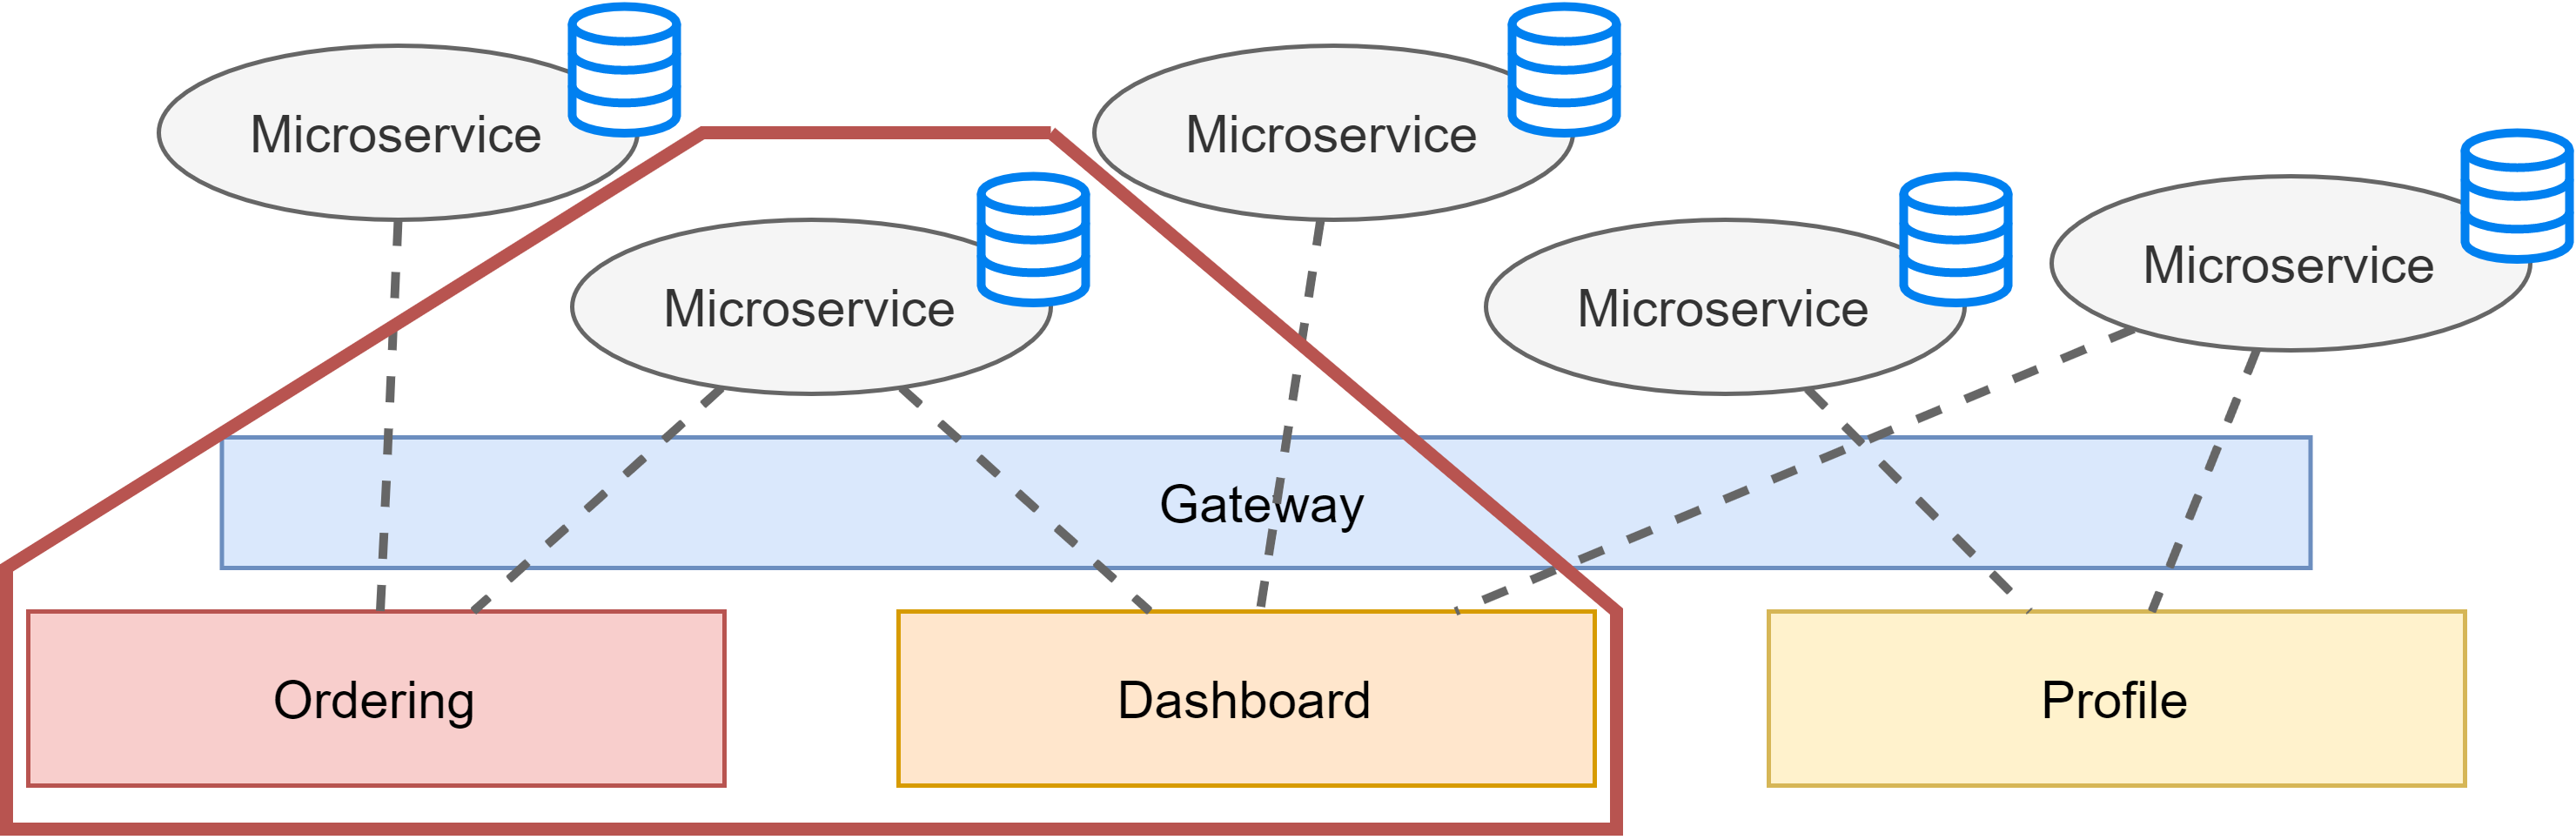
\includegraphics[width=\textwidth, keepaspectratio]{no-bff.png}
    \caption{Outline the coupling between \ac{MF}, if \ac{BFF} pattern is not used \cite{Leitner.2020}}
    \label{img:team_slicing_no_bff}
\end{figure}

The scenario shown in Figure \ref{img:team_slicing_no_bff} is, that one microservice is used by multiple \acp{MF}.
One instance is outlined in Red.
Assuming the microservice provides a service via some form over a gateway, both \acp{MF} will break, when the \ac{API} changes.
Hence, this creates an unwanted coupling between \textit{Ordering}, \textit{Dashboard} and the microservice.
As a result, the autonomy aspect between these parties is broken.

Before explaining how to fix the problem, first is important how the \ac{BFF} pattern can be translated to work with \ac{MFA}.
This is shown in Figure \ref{img:team_slicing_bff}.
Each \ac{MF} gets its own microservice and it is the only communication channel from the \ac{MF} to the backend.
Therefore, the \ac{BFF} microservice provides the \ac{API} for the \ac{MF} and handles all the communication with multiple microservices.
As a result, the \ac{MF} and \ac{BFF} microservice is considered to be one unit and the same team must be responsible for both \cite{Leitner.2020}.

\begin{figure}[h]
    \centering
    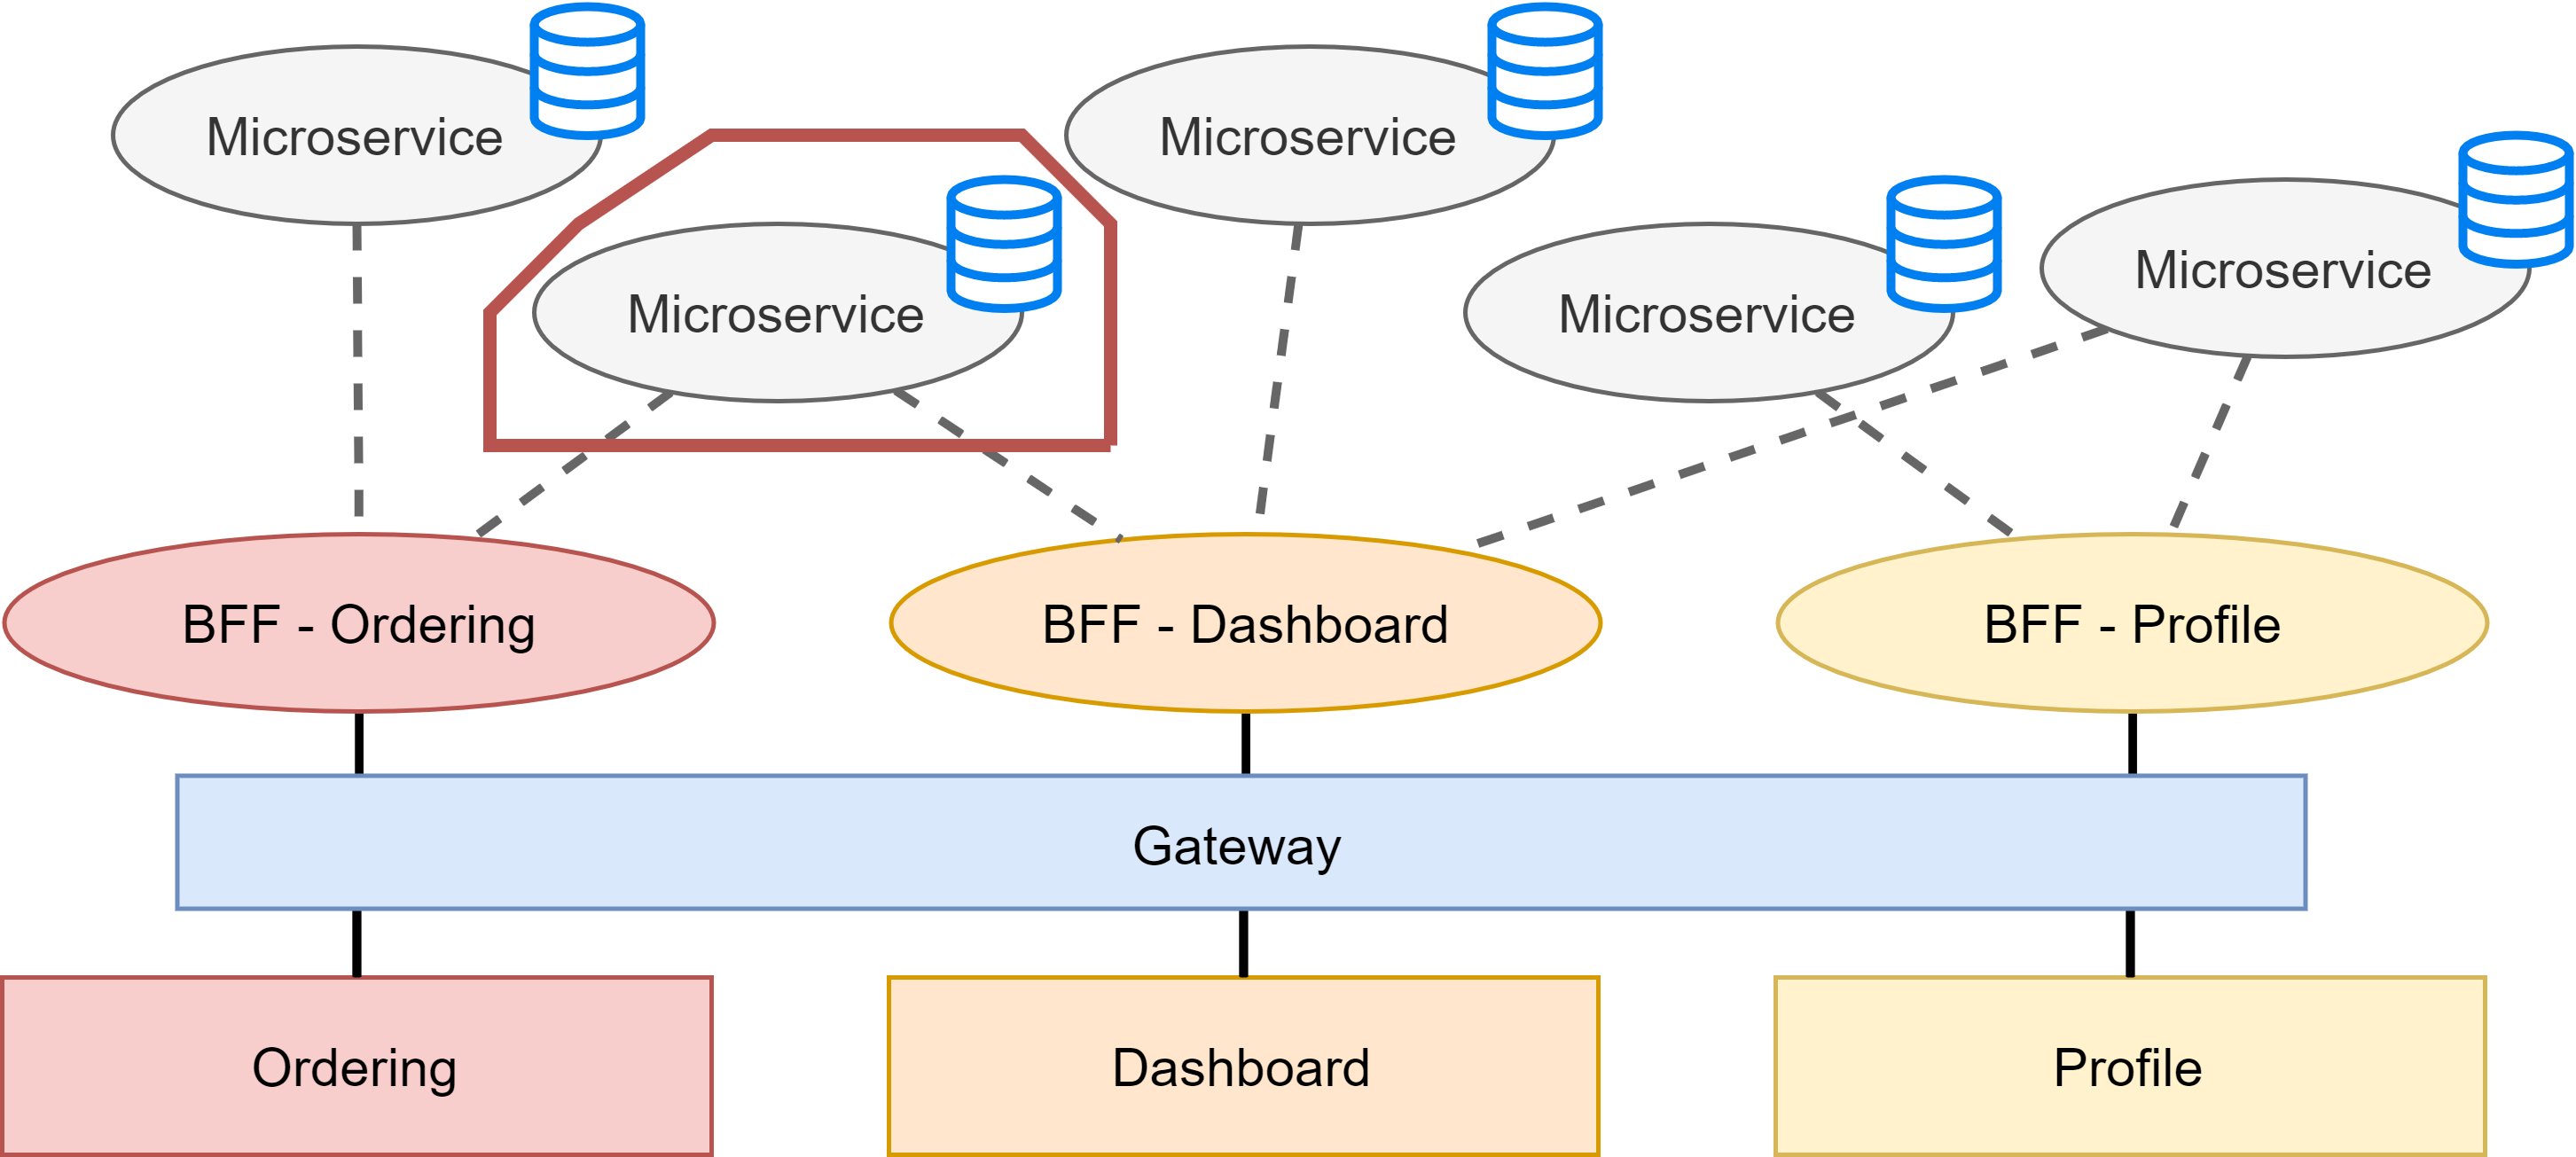
\includegraphics[width=\textwidth, keepaspectratio]{bff.png}
    \caption{Using the \ac{BFF} architecture in combination with the \ac{MFA} \cite{Leitner.2020}}
    \label{img:team_slicing_bff}
\end{figure}

The coupling problem is solved with the \ac{BFF} pattern, because there is a clear responsibility cut between the \ac{MF} and its \ac{BFF} micro frontends to the shared microservice.
This approach was mentioned by \textcite{Jackson.2019}, \textcite{Leitner.2020} and \textciteRehm{}.

There are different interpretations on how much responsibility the dedicated microservice should have.
\textcite{Leitner.2020} suggests that it is only used to accumulate and provide information for the \ac{MF}.
By contrast, \textcite{Jackson.2019} does not restrict the responsibility of the dedicated microservice.
However, both agree that one team should be responsible for the micro frontend and its dedicated microservice.

Using the \ac{BFF} architecture is not required in order to use \acp{MF}, instead it is an extension and has both advantages and disadvantages.
An important advantage is that it simplifies sharing microservices between multiple \acp{MF} without creating unwanted coupling between \acp{MF} and microservices.
However, adding a new microservice adds complexity to the overall system.



\paragraph{Micro frontend composition}\label{cha:theroy_extensions_composition}

Another aspect to outline about \ac{MFA} is the composition part.
Three approaches are commonly outlined, which are shown in Figure \ref{img:compositions}.
The first one is to show one \ac{MF} per page (left).
This is considered as the default approach and is the simplest approach compared to the other approaches.
Next is to show multiple \acp{MF} per page (middle).
In this case, each \ac{MF} is placed into its own node and there is a clear boundary between them.
This requires some form of templating, which is addressed in the \textit{\nameref{cha:requirement_detail_integration_pagelayout}} requirement.
Finally, the widget approach can be seen at the right.
It allows each \ac{MF} to share components with other \acp{MF} and they can be included by \acp{MF} as needed.
How to implement it is discussed in the \textit{\nameref{cha:requirement_detail_integration_widget}} requirement.
One combination that was not mentioned in the literature research, is to combine widgets and multiple \acp{MF} per page.
Although this is possible, no practical scenario is mentioned where it is needed.

\begin{figure}[h]
    \centering
    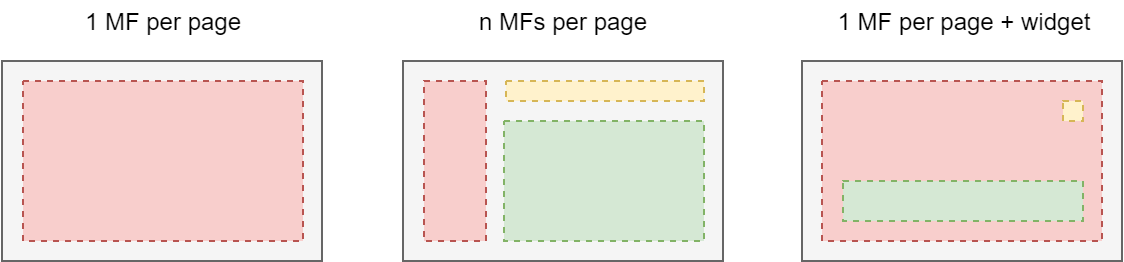
\includegraphics[width=\textwidth, keepaspectratio]{compositions.png}
    \caption{Different \ac{MF} composition approaches}
    \label{img:compositions}
\end{figure}



\section{Micro frontend practical parts}\label{cha:theory_practic}

Before concluding the \ac{MF} fundamentals, there are some topics worth mentioning, because they come up in the chapter \ref{cha:requirement}.



\paragraph{Bundle size}

A term used multiple times in the chapter \ref{cha:requirement} is bundle size.
It refers to the entire size of the application's \ac{JS} bundle.
It is relevant, because a \ac{MF} application consists of many \ac{MF} and each is bundled separately.
This can result in a lot of data which is required for the application.



\paragraph{Duplicate requrests}

As shown in the \nameref{cha:theory_extensions_bff} paragraph, \acp{MF} should be independent and there are scenarios where two \acp{MF} need data from the same microservice.
If the implementation strongly follows the concept of \ac{MFA}, then each \ac{MF} fetches the data on their own.
However, this can result in a poor \ac{UX}.
Therefore, there are approaches which tackle this issue, with the expense of autonomy.
This is mainly addressed in the \hyperref[cha:requirement_detail_performance]{Performance} requirement \cite{Steyer.2019}.



\paragraph{Custom Events}\label{cha:theory_practice_customevents}

Custom Events is a browser native feature to emit events on a node in the \ac{DOM} and listen for them.
A Custom Event consists of a name and any data which is added to it.
To emit it, a \ac{HTML} element is needed as host.
Any \ac{JS} code can listen on any \ac{HTML} element for events which are emitted on this particular element\footnotemark.
\footnotetext{\url{https://developer.mozilla.org/en-US/docs/Web/Guide/Events/Creating_and_triggering_events} (Visited on 09/02/2020)}



\paragraph{\acl{CDC} testing}\label{cha:theory_practice_cdctesting}

\ac{CDC} testing is about abstracting the communication between two parties to test them in isolation of each other.
This implies, that only one of both is needed in order to test the communication at a time.
Hence, each party is responsible to validate these tests before deployment to ensure that a build is working according to the contract.
A contract is either created by hand or via a tool\footnotemark.
\footnotetext{\url{https://www.martinfowler.com/articles/consumerDrivenContracts.html} (Visited on 02/09/2020)}
A common tool for such tests in a microservice environment was mentioned by \textcite{Laug.2018}, which is \textit{pact.io}.
This tool simplifies the automation process of such tests.



\paragraph{Web Components}\label{cha:theory_practice_webcomponent}

Web Components is a native browser feature which consists of \textit{Custom elements}, \textit{Shadow \ac{DOM}} and \textit{\ac{HTML} templates}.
\textit{Custom elements} is a \ac{JS} \ac{API} to create reusable custom components and define their behavior for a web page.
Such a \textit{Custom element} requires a tag name, which must include a dash by convention.
A tag name can only exist once per page\footnotemark{}.
\footnotetext{\url{https://developer.mozilla.org/en-US/docs/Web/Web_Components} (Visited on 09/02/2020)}
Furthermore, the \textit{Custom element} \ac{JS} \ac{API} provides the ability to either pass information into the custom element via \ac{HTML} attributes or \ac{JS} properties.
The first can be achieved by adding the attribute into the custom element tag in the \ac{HTML}.
Contrary to that, the latter needs \ac{JS} to retrieve the custom component node from the \ac{DOM} in order to access its properties via methods from the custom component\footnotemark.
\footnotetext{\url{https://developers.google.com/web/fundamentals/web-components/customelements\#properties_and_attributes} (Visited on 09/02/2020)}

An optional feature of a \textit{Custom element} is the \textit{Shadow \ac{DOM}}.
The \textit{Shadow \ac{DOM}} is a \ac{JS} \ac{API} to attach a virtual \ac{DOM} to the actual \ac{DOM}, hence the name \textit{shadow}.
These elements are rendered separately from the actual \ac{DOM}.
It also allows to encapsulate \ac{CSS} styles within itself.
As a result, the main page is only able to style the \ac{CSS} via variables, while the styles from within the \textit{Shadow \ac{DOM}} do not affect the main page\footnotemark{}.
\footnotetext{\url{https://developers.google.com/web/fundamentals/web-components/shadowdom\#stylefromoutside} (Visited on 09/02/2020)}

Lastly, there are \textit{\ac{HTML} templates}, which provide the \textit{template} and \textit{slot} tag.
Only the \textit{slot} tag is required later on in chapter \ref{cha:requirement}.
It is a placeholder within the Web Component that can be filled with any markup from within the main page\footnotemark.
\footnotetext{\url{https://developer.mozilla.org/en-US/docs/Web/HTML/Element/slot} (Visited on 09/02/2020)}





\section{Conclusion}

To conclude the \ac{MF} fundamentals, there are some important hints about \acp{MF} in general.
The first is from \textcite{Laug.2018b} who points out, that \ac{MFA} does not increase the development speed, but rather sustains it.
He mentions, that this is a common misconception of the micro architectures.
Secondly, \textcite{Leitner.2020} believes that no more than 20\% of projects actually need the \ac{MFA}.
He continues, that the \ac{MFA} adds a lot of complexity, which must be worth it for the project in order to use \ac{MFA}.
Finally, \textcite{Steyer.2019} came up with a simple decision tree to find out if a project even needs this architecture, which is shown in Figure \ref{img:decision_tree}.
The tree starts on the left side and, based on it, only in a specific case the architecture is recommended.
More about the criteria for a \ac{MF} application is described in section \ref{cha:scenarios_criteria}.

\begin{figure}[h]
    \centering
    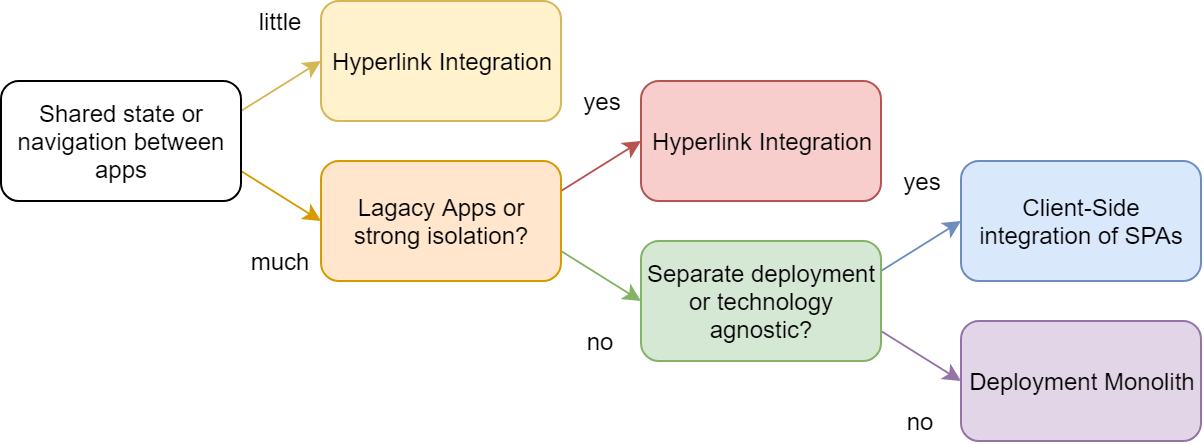
\includegraphics[width=\textwidth, keepaspectratio]{decition_tree.png}
    \caption{Decision tree from \ac{MFA} which can be used to determine which type of architecture or implementation should be used \cite{Steyer.2019}}
    \label{img:decision_tree}
\end{figure}

This sums up the \ac{MF} fundamentals chapter and the next chapter is about when to use the \ac{MFA}.


